
\nomenclature[F]{$n$}{Drehzahl \nomunit{$\frac{1}{\text{min}}$}}

\newvideofile{gleichstrommaschine}{Gleichstrommaschine}
\section{Gleichstrommaschine}
\s{
	Gleichstrommaschinen sind Elektromaschinen, die mit Gleichstrom betrieben werden und sowohl als Motoren als auch als Generatoren verwendet werden können. Sie zeichnen sich durch eine präzise Steuerbarkeit der Drehzahl und des Drehmoments aus, was sie ideal für Anwendungen mit variabler Geschwindigkeit und Last macht. Gleichstrommaschinen haben einen hohen Anlaufdrehmoment und ermöglichen eine einfache Umkehrung der Drehrichtung. Sie werden häufig in Elektrofahrzeugen, industriellen Steuerungsanlagen und batteriebetriebenen Geräten eingesetzt.
}

\begin{frame}\ftx{Gleichstrommaschine Vorteile / Nachteile}
	\begin{minipage}{0.45\textwidth}
	\textbf{Vorteile:}
	\begin{itemize}
		\item Einfacher und kostengünstiger \\ Aufbau der Stromrichter
		\item Hohe Regeldynamik
		\item Direkter Betrieb der Maschine mit \\ Akkumulatoren möglich
		\item Große Überlastfähigkeit
	\end{itemize}\pause
	\end{minipage}\hfill 
	\raisebox{3ex}{
	\begin{minipage}{0.45\textwidth}
	\textbf{Nachteile:}
	\begin{itemize}
		\item Hoher Konstruktionsaufwand
		\item Wartungsintensiv (Bürsten)
		\item Geringe Leistungsdichte
		\item Kosten
	\end{itemize}
	\end{minipage}
	}
	\speech{Gleichstrommaschine1}{1}{Die Gleichstrommaschine wird zum Beispiel in großer Anzahl bei einfachen batteriebetriebenen Geräten oder im Kraftfahrzeug eingesetzt. Ein Vorteil der Maschine ist der einfache Aufbau der Stromrichter um die Drehzahl der Maschine einstellen zu können. Die Regeldynamik, also die Geschwindigkeit der Drehzahlregelung, kann dabei sehr hoch sein. Auch ist ein direkter Betrieb ohne jegliche Elektronik an Batterien möglich, was bei sehr einfachen Geräten wie zum Beispiel Spielzeugen ein großer Vorteil ist.}
	\speech{Gleichstrommaschine1}{2}{Ein wesentlicher Nachteil der Gleichstrommaschine ist der hohe Konstruktionsaufwand und die damit verbundenen hohen Kosten. Die Leistungsdichte ist durch den Aufbau deutlich geringer als bei den anderen Maschinentypen. Ein weiterer wesentlicher Nachteil ist der Verschleiß der zwingend notwendigen Bürsten, die eine regelmäßige Wartung oder wenn das nicht möglich ist, eine geringe Lebensdauer bedeuten.}
\end{frame}

\begin{frame} \ftx{Elektrische Maschinen}
	\subsection{Exkurs Prinzip des Elektromotors\label{KapExkursLorentz}}
	\s{	
		Zu Beginn werden die im Modul 6 vorgestellten Prinzipien aufgefrischt. Die Abbildung \ref{AbbLorentzSchleife} zeigt in drei Schaubildern kurzgefasst die Wirkweise eines Elektromotors. Zum grundlegenden Aufbau eines Elektromotors gehören ein feststehender Teil, Ständer\index{Ständer} oder Stator\index{Stator} genannt, und ein sich drehender Teil, auch Läufer\index{Läufer} oder Rotor\index{Rotor} genannt.
		In den drei Abbildungen ist eine Leiterspule in einem Hufeisenmagnet zu sehen. Der Hufeisenmagnet bildet hier den Strator und eine um die eigene Achse bewegliche Leiterspule stellt den Rotor dar. 
		Das erste Schaubild illustriert den isolierten Verlauf der magnetischen Feldinien des Hufeisenmagnets. Sie verlaufen innerhalb des Hufeisenmagneten vertikal von Nord- zum Südpol. 
		Das zweite Schaubild zeigt den isolierten Verlauf der magnetischen Feldlinien der stromdurchflossen Leiterschleife. Durch den Stromfluss entstehen an der Leiterschleife zwei entgegenwirkende Wirbelfelder. 
		Im dritten Schaubild wird die Wechselwirkung des Hufeisenmagneten (Statorfeld) und der stromdurchflossenen Leiterschleife (Rotorfeld) aufgezeigt. Die beiden Felder überlageren sich. Die aus der Überlagerung resultierende Lorentzkraft bringt gemäß der Rechten-Hand-Regel die Leiterschleife zum rotieren. Aus der elektromagnetischen Energie entsteht mechanische Energie.
	}
	\fu{
		\begin{minipage}{0.25\textwidth}
			\foo{width=0.9\textwidth}{width=0.9\textwidth}{Lorentzkraft_Feldverlaeufe5}{
				\put(85, 78){\color{magnetfeld}N}
				\put(85, 15){\color{magnetfeld}S}
			}{}
		\end{minipage}
		\hfill
		\begin{minipage}{0.25\textwidth}
			\foo{width=0.9\textwidth}{width=0.9\textwidth}{Lorentzkraft_Feldverlaeufe6}{
				\put(5, 46.5){\color{magnetfeld}N}
				\put(55, 46.5){\color{magnetfeld}S}
				\put(-35, 47){\color{gray}+}
			}{}
		\end{minipage}
		\hfill
		\begin{minipage}{0.25\textwidth}
			\foo{width=0.9\textwidth}{width=0.9\textwidth}{Lorentzkraft_Feldverlaeufe7}{
				\put(85, 78){\color{magnetfeld}N}
				\put(85, 15){\color{magnetfeld}S}
				\put(8, 52){\color{gray}$F$}
				\put(54, 42){\color{gray}$F$}
				\put(-35, 47){\color{gray}$\Rightarrow$}
			}{}
		\end{minipage} 
	}{{\bf Prinzip des Elektromotors.} Die Lorentzkraft bringt die sich im Magnetfeld befindende stromdurchflossene Leiterschleife in eine Drehbewegung. \label{AbbLorentzSchleife}}

	\s{Die Lorentzkraft kann mit der aus Modul 6 bekannten Formel berechnet werden:}
	\begin{eq}
		F =B\cdot I\cdot \ell\cdot N
	\end{eq}

\end{frame}

\begin{frame} \ftx{Beispiel: Kraft einer Gleichstrommaschine}
	\begin{bsp}{Kraft einer Gleichstrommaschine}{}
		Ein Gleichstrommotor hat im Luftspalt eine magnetische Flussdichte von $B=0,8\,\mathrm{T}$. Unter den Polen befinden sich insgesamt $N=400$ Ankerdrähte, die mit einem Strom von $I=10\,\mathrm{A}$ durchflossen werden. Die wirksame Leiterlänge ist $\ell=150\,\mathrm{mm}$.

		Berechnen Sie die Kraft $F$ am Umfang des Ankers.\pause
		\begin{align*}
			F & =B\cdot I\cdot \ell\cdot N\\
			  & =0,8\,\frac{\mathrm{Vs}}{\mathrm{m}^2}\cdot 10\,\mathrm{A}\cdot0,15\,\mathrm{m}\cdot 400\\
			  & =480\,\frac{\mathrm{kg}\cdot\mathrm{m}^2\cdot\mathrm{s}\cdot\mathrm{A}\cdot\mathrm{m}}{\mathrm{s}^3\cdot\mathrm{A}\cdot\mathrm{m}^2} = 480\,\mathrm{N}		
		\end{align*}

	\end{bsp}
\end{frame}

\s{
	\subsection{Aufbau und Gehäusekonstruktion}\index{Gleichstrommaschine>Aufbau}
}
\begin{frame}\ftx{Aufbau}
	\s{
		Der Aufbau der Gleichstrommaschine wird anhand dreier Abbildungen dargestellt. Abbildung \ref{GrafikGleichstrommaschine} zeigt ein diagonales Schnittmodell der Gleichstrommaschine, das eine allgemeine Übersicht über die Komponenten von Stator und Rotor gibt. Zur detailierteren Veranschaulichung des Aufbaus werden die Abbildung \ref{QuerschnittGleichstrommaschine} mit Fokus auf dem Stator und Abbildung \ref{FotoRotor} zur Veranschaulichung des Rotors einer Gleichstrommaschine herangezogen. 

		\nomenclature[F]{$p$}{Polpaarzahl}
	}
	\fo{width=0.6\textwidth}{height=0.85\textheight}{gleichstrommaschine1}{
		\put(70,0){\line(-1,1){38}}\put(70.3,0){Kommutatorlamellen}
		\put(86,8){\line(-1,1){56}}\put(86.3,8){Erregerpole mit Wicklung}
		\put(90,16){\line(-1,1){45}}\put(90,16){Wicklungen des Rotors}
		\put(95,24){\line(-1,1){28}}\put(95.3,24){Rotorzylinder}
		\put(105,32){\line(-1,1){28}}\put(105.3,32){Lager}
	}{{\bf Grafik einer aufgeschnittenen Gleichstrommaschine.}  \label{GrafikGleichstrommaschine}}
\end{frame}
	

\begin{frame}\ftx{Aufbau}
	\fo{width=0.8\textwidth}{height=0.85\textheight}{Aufbau1}{
		\put(27,20){\line(1,1){16}}\put(-5,20){Wendepole mit Wicklung}
		\put(30.5,15){\line(1,1){22}}\put(-5,15){Rotorzylinder mit Wicklung}
		\put(40,5){\line(1,1){17}}\put(9.5,5){Kompensations\-wicklung}
		\put(40.5,0){\line(1,1){14}}\put(9.5,0){Pol mit Erregerwicklung}
		\put(85,5){\line(-1,1){14}}\put(85.3, 5){Polschuh}
		\put(85,0){\line(-1,1){8}}\put(85.3,0){Ständerjoch}
	}{{\bf Grundlegender Aufbau einer Gleichstrommaschine.} Hier mit nur einem Polpaar (Polpaarzahl $p=1$). \label{QuerschnittGleichstrommaschine}} 
	\s{	
		Die Komponenten des Strators, auch Ständer genannt, werden im frontalen Querschnitt einer Gleichstrommaschine (Abbildung \ref{QuerschnittGleichstrommaschine}) gut veranschaulicht. Eine der grundlegende Komponente ist die Erregerwicklungen \index{Erregerwicklung}, die um ein Polschuh gewunden, einen Pol darstellt. Die Pole haben die Aufgabe, ein Magnetfeld, Erregerfeld genannt, zu erzeugen.

		Da ein magnetisches Feld immer einen Nord- und einen Südpol beinhaltet, werden die Pole paarweise gegenüber eingebaut. Die daraus resultierende Kenngröße, die Polpaarzahl, gibt Aufschluss über die Betriebseigenschaften der Gleichstrommaschine. 
		Eine höhere Polpaarzahl verringert die Drehzahl, erhöht jedoch das Drehmoment. Bei Kleinstmaschinen können die Erregerwicklungen durch Permanentmagnete ersetzt werden. 
		Bei größeren Maschinen (ca. über 1 kW) sind zusätzlich Wendepolwicklungen vorhanden, die hier jedoch vernachlässigt werden.
	}
\end{frame}

\begin{frame} \ftx{Rotor und Kommutator}
	\s{	
		In der Abbildung \ref{FotoRotor} sind die Komponenten des Rotors gut ersichtlich. Im Allgemeinen wird der Rotor auch Anker oder als Läufer bezeichnet. Die Funktion des Rotors beteht dahin die elektromagnetische Energie durch Rotationen um die eigene Achse in mechanische Energie (und umgekehrt) zu wandlen. 
		Hierzu ist der Rotor an einer Motorwelle befestigt, die die mechanische Energie überträgt. Das Kugellager am Ende der Motorwelle verringert dabei die Reibungsverluste bei der Energieübertragung. 
		Um den Rotor in Bewegung zu bringen, ist das Zusammenwirken von Kommutator und Rotorwicklung wichtig. Die Rotorwicklung, auch Ankerwicklung bezeichnet, hat die Aufgabe ein magnetisches Feld, das Ankerfeld, zu erzeugen. Erst durch die Interaktion des Ankerfelds mit dem Erregerfeld wird ein Drehmoment auf den Rotor ausgeübt und setzt diesen in Bewegung. 
		Die Blechwände, um die die Spulen gewickelt sind, bestehen aus isolierenden Blechen, um Wirbelströme in den Wicklungen zu reduzieren. 
		Der Kommutator\index{Kommutator} oder Stromwender\index{Stromwender} hat die Funktion die Rotorwicklung getaktet mit Storm zu versorgen. Er besteht aus mehrenen voneinanderen getrennte Lamellen, die jeweils mit einem Strang der Rotorwicklung verbunden. 
		Der Strom wird nun über am Strator angebrachten Kohlebürsten an die Kommutatorlamellen geleitet. Durch die Drehung der Lamellen unter den Bürsten wirkt der Kommutator als mechanischer Schalter und sorgt dafür, dass die Stromrichtung in den Rotorwicklungen die sich jeweils unter den Hauptpolen befinden gleich bleibt.
	}
	\fo{width=0.8\textwidth}{width=0.75\textwidth}{Rotor_Gleichstrommaschine_kl}{
		\put(87,45){\line(-1,1){10}}\put(87,45){Welle}
		\put(65,20){\line(-1,1){10}}\put(65.3,20){Blechpaket}
		\put(48,10){\line(-1,1){10}}\put(48,10){Wicklungen}
		\put(35,5){\line(-1,1){10}}\put(35.3,5){Kommutator}
		\put(23,0){\line(-1,1){10}}\put(23.3,0){Lager}
	}{{\bf Foto eines Rotors.} Zu erkennen sind hier die charakteristischen Bauelemente. \index{Gleichstrommaschine>Rotor}\label{FotoRotor}}  
\end{frame}

\s{\subsection{Magnetische Felder}\index{Gleichstrommaschine>Felder}}
\begin{frame}\ftx{Erregerfeld}
	\s{Für die Lorentzkraft ist das magnetische Feld entscheidend, in dem sich der Leiter bewegt. Dieses Feld wird durch den Stator mit den Erregerwicklungen erzeugt und ist im Bereich des Rotors näherungsweise parallel und homogen.
	}
	\fo{width=0.6\textwidth}{height=0.85\textheight}{Erregerfeld}{
		\put(50,97){\color{magnetfeld}\makebox[0pt]{N}}
		\put(50,0){\color{magnetfeld}\makebox[0pt]{S}}
	}{{\bf Erregerfeld einer Gleichstrommaschine.} Schematische Darstellung in der Vorderansicht.}	
\end{frame}
 

\begin{frame}\ftx{Induzierte Spannung}
\s{\subsection{Berechnung des Drehmoments}}
	\s{
		In Modul 6 und Kapitel \ref{KapExkursLorentz} ist bereits die Kraftwirkung auf einen stromdurchflossenen Leiter im Magnetfeld erklärt worden. Um das Drehmoment der Gleichstrommaschine zu berechnen, wird zuerst die induzierte Spannung ermittelt (siehe Modul 6). Dreht sich der Rotor einer erregten Gleichstrommaschine, wird in jeder Leiterschleife des Ankers eine Spannung induziert. Nach dem Induktionsgesetz (Gleichung \ref{GlInduktionsgesetz}) ist die Höhe der induzierten Spannung (Quellenspannung) $U_\mathrm{q}$ vom magnetischen Fluss $\varPhi$ und der zeitlichen Änderung, in diesem Fall der Drehzahl $n$ bzw. der damit verküpften Kreisfrequenz $\omega = 2\pi\cdot n$ abhängig.
		Werden hierzu noch die spezifischen geometrischen Gegebenheiten des Rotors in Form der Ankerkonstanten $K$ multipiziert, so ergibt das Produkt aus diesen Kenngrößen die induzierte Spannung $U_\mathrm{q}$ der Gleichstrommaschine (siehe Gleichung \ref{GlInduzierteSpannungGM})
	}

	\begin{eq}
		U_\mathrm{q} = K \cdot \varPhi \cdot \omega \label{GlInduzierteSpannungGM}
	\end{eq}
	\b{
		\begin{itemize}
		\item Induzierte Spannung (Quellenspannung): $U_\mathrm{q}$ [V]
		\item Ankerkonstante: $K$ [1]\index{Ankerkonstante} \nomenclature[F]{$K$}{Ankerkonstante der Gleichstrommaschine}
		\item Fluss: $\varPhi$ [Vs]
		\item Winkelgeschwindigkeit: $\omega_\mathrm{mech}$ [rad/s]
	\end{itemize}	
	}	\pause
	
	\s{ 
		Wenn sowohl die elektrischen als auch mechanischen Verluste vernachlässigt wird, kann die induzierte Spannung kann auch direkt über die sogenannte innere Leistung $P_\mathrm{i}$ angegeben werden. Diese entspricht dann sowohl der elektrischen Leistung $U_\mathrm{q}\cdot I_\mathrm{A}$, als auch der mechanischen Leistung $P_\mathrm{mech}$, welche sich aus dem Produkt des inneren Drehmoments $M_\mathrm{i}$ und der Winkelgeschwindigkeit $\omega$ errechnet.
	}
	\begin{eq}
		P_\mathrm{i} = U_\mathrm{q}\cdot I_\mathrm{A} =  P_\mathrm{mech} = M_\mathrm{i}\cdot \omega \label{GlGMWirkungsgrad}
	\end{eq}

	\b{
		\begin{itemize}
			\item innere elektrische Leistung: $P_\mathrm{i}$ [W]
		\end{itemize}
	}
\end{frame}
	
\begin{frame}\ftx{Inneres Moment}
	\s{Wird diese Erkenntnis nun in Gleichung \ref{GlInduzierteSpannungGM} eingesetzt, errechnet sich das inner Drehmoment $M_\mathrm{i}$ aus dem Produkt der Ankerkonstante $K$, den magnetischen Fluss $\varPhi$ und dem Ankerstrom $I_\mathrm{A}$}	
	\begin{eq}
		M_\mathrm{i} = K \cdot \varPhi \cdot I_\mathrm{A} \label{GlMomentGM} 
	\end{eq}
	\b{
		\begin{itemize}
			\item Inneres elektrisches Moment:  $M_\mathrm{i}$ [Nm]
			\item Ankerkonstante: $K$ [1]
			\item Fluss: $\varPhi$ [Vs]
			\item Ankerstrom: $I_\mathrm{A}$  [A]
		\end{itemize}\pause
	}
	\s{
		Im Motorbetrieb ist das Drehmoment an der Welle der Maschine das innere Drehmoment $M_\mathrm{i}$ abzüg\-lich der Verluste $M_\mathrm{V}$. Das Maschinenmoment kann auch durch den Wirkungsgrad $\eta_1$ ausgedrückt werden. Dieser Wirkungsgrad vernachlässigt allerdings die elektrischen Verluste durch den Ankerwiderstand und der Erregung.
	}
	\begin{eq}
		M = M_\mathrm{i} - M_\mathrm{V}\qquad \qquad M = \eta_1\cdot M_\mathrm{i}\label{GLMomentWirkungsgradGM}
	\end{eq}
	\begin{itemize}
		\item Verlustmoment: $M_\mathrm{V}$ [Nm]
		\item Wirkungsgrad:  $\eta$ [1]
	\end{itemize}

\end{frame}




\s{\subsection{Fremderregte Gleichstrommaschine}}
\begin{frame}\ftx{Fremderregte Gleichstrommaschine}
	\s{Der Erregerkreis im Stator der Gleichstrommaschine und der Rotorkreis, der über den Kommutator mit Strom versorgt wird, sind prinzipiell unabhängig voneinander. Wenn beide Stromkreise von unterschiedlichen Spannungsquellen versorgt werden, wird die Maschine fremderregt genannt. \index{Gleichstrommaschine>Fremderregt} Das Ersatzschaltbild ist in Abbildung \ref{AbbGMFremderregt} dargestellt.}
	\fu{
		\begin{circuitikz}
    \draw (0,0) to[short, o-] (4,0) -- (4,1.5) to[L=$L_\mathrm{E}$] (2,1.5) to[R=$R_\mathrm{E}$, i<_=$I_\mathrm{E}$, -o] (0,1.5) to[open, v=$U_\mathrm{E}$] (0,0);
    \draw (5,1.5) node[elmech](GM){GM};
    \draw (GM.north) -- (5,3) -- (6,3) to[R=$R_\mathrm{A}$, i=$I_\mathrm{A}$, -o] (8,3) to[open, v=$U_\mathrm{A}$] (8,0)
    (GM.south) -- (5,0) to[short, -o] (8,0)
    (6,3) to[open, v=$U_\mathrm{q}$] (6,0);
\end{circuitikz}
	}{{\bf Ersatzschaltbild einer fremderregten Gleichstrommaschine.} \label{AbbGMFremderregt}}
	\s{Der Erregerkreis besteht aus der Induktivität der Erregerwicklung $L_\mathrm{E}$ und dem Kupferwiderstand $R_\mathrm{E}$ der Spule. Im Ankerkreis wird die Wicklung als Kreis mit angedeuteten Schleifringen dargestellt, da sie einerseits eine Induktivität, als auch eine Spannungsquelle darstellt. Auch der Anker hat einen ohmschen Widerstand $R_\mathrm{A}$.
	
	Der Maschenumlauf im Rotorkreis ergibt:}
	\begin{eq}
		U_\mathrm{A} = U_\mathrm{q} + I_\mathrm{A}\cdot R_\mathrm{A}
	\end{eq}
	
	\s{Durch Einsetzen von Gleichung \ref{GlInduzierteSpannungGM} und \ref{GlMomentGM} ergibt sich die Drehzahl/Drehmoment- und Ankerstromkennlinie für die fremderregte Gleichstrommaschine:}
	\s{
		\begin{eq}
			n = \frac{U_\mathrm{A}}{2\pi K\cdot \varPhi} - \frac{R_\mathrm{A}\cdot M_\mathrm{i}}{2\pi(K\cdot \varPhi)^2}\label{GlfremderregteGM1}
		\end{eq}
	}
	\b{
		\begin{eq}
			n = \frac{U_\mathrm{A}}{2\pi K\cdot \varPhi} - \frac{R_\mathrm{A}\cdot M_\mathrm{i}}{2\pi(K\cdot \varPhi)^2}
			\qquad \qquad I_\mathrm{A} = \frac{M_\mathrm{i}}{K\cdot \varPhi}
		\end{eq}
	}
\end{frame}


\begin{frame}\ftx{Beispiel: Fremderregte Gleichstrommaschine}
	\s{
		\begin{bsp}{Fremderregte Gleichstrommaschine}{}
			Eine fremderregte Gleichstrommaschine mit der Ankerkonstante $K=\frac{1}{2\pi}$ hat bei der Spannung $U_\mathrm{A}=400\,\text{V}$ eine Leerlaufdrehzahl von $n=1200\,\frac{1}{\text{min}}$. Der Ankerwiderstand beträgt $R_\mathrm{A}=2,3\,\Omega$. 
			\begin{itemize}
				\item [a)] Wie groß ist der Erregerfluss $\varPhi$?
				
				Im Leerlauf ist das innere Moment $M_\mathrm{i}$ gleich Null. Gleichung \ref{GlfremderregteGM1} vereinfacht sich daher zu:
				\begin{align*}
					n&=\frac{U_\mathrm{A}}{2\pi K\cdot \varPhi}\\
					\varPhi&=\frac{U_\mathrm{A}}{2\pi K\cdot n} = \frac{400\,\text{V}}{\frac{2\pi}{2\pi}\cdot 1200 \,\frac{1}{\text{min}}\cdot \frac{1}{60\,\frac{\text{s}}{\text{min}}}}  = 20\,\text{Vs}
				\end{align*}
				
				\item[b)] Wie schnell dreht die Maschine bei einem inneren Drehmoment von $M_\mathrm{i}=10\,\text{Nm}$?
				\begin{align*}
					n &= \frac{U_\mathrm{A}}{2\pi K\cdot \varPhi} - \frac{R_\mathrm{A}\cdot M_\mathrm{i}}{2\pi(K\cdot \varPhi)^2}\\
					 &= \frac{400\,\text{V}}{\frac{2\pi}{2\pi}\cdot 20\,\text{Vs}} - \frac{2,3\,\Omega \cdot 10\,\text{Nm}}{2\pi(\frac{1}{2\pi}\cdot 20\,\text{Vs})^2}\\
					 &= 20\,\frac{1}{\text{s}} - 0,362 \,\frac{1}{\text{s}} = 19,638\,\frac{1}{\text{s}} =  1178,3\,\frac{1}{\text{min}}
				\end{align*}
				\item[c)] Wie groß ist der Ankerstrom?
				\begin{align*}
					I_\mathrm{A} &= \frac{M_\mathrm{i}}{K\cdot \varPhi} = \frac{10\,\text{Nm}}{\,\frac{1}{2\pi}\cdot 20\,\text{Vs}\,} = 3,61\,\text{A}
				\end{align*}
			\end{itemize}
		\end{bsp}
	}
	\b{
		Eine fremderregte Gleichstrommaschine mit der Ankerkonstante $K=\frac{1}{2\pi}$ hat bei der Spannung $U_\mathrm{A}=400\,\text{V}$ eine Leerlaufdrehzahl von $n=1200\,\frac{1}{\text{min}}$. Der Ankerwiderstand beträgt $R_\mathrm{A}=2,3\,\Omega$. 
		\begin{itemize}
			\item [a)] Wie groß ist der Erregerfluss $\varPhi$? \pause	
					
				Im Leerlauf ist das innere Moment $M_\mathrm{i}$ gleich Null. Der lastabhängige Drehzahlabfall entfällt daher:
				\begin{align*}
					n&=\frac{U_\mathrm{A}}{2\pi K\cdot \varPhi}\\
					\varPhi&=\frac{U_\mathrm{A}}{2\pi K\cdot n} = \frac{400\,\text{V}}{\frac{2\pi}{2\pi}\cdot 1200 \,\frac{1}{\text{min}}\cdot \frac{1}{60\,\frac{\text{s}}{\text{min}}}}  = 20\,\text{Vs}
				\end{align*}
		\end{itemize}	
	}
\end{frame}
\b{
	\begin{frame}\ftx{Beispiel}
		\begin{itemize}
			\item[b)] Wie schnell dreht die Maschine bei einem inneren Drehmoment von $M_\mathrm{i}=10\,\text{Nm}$?\pause
				\begin{align*}
					n &= \frac{U_\mathrm{A}}{2\pi K\cdot \varPhi} - \frac{R_\mathrm{A}\cdot M_\mathrm{i}}{2\pi(K\cdot \varPhi)^2}\\
					&= \frac{400\,\text{V}}{\frac{2\pi}{2\pi}\cdot 20\,\text{Vs}} - \frac{2,3\,\Omega \cdot 10\,\text{Nm}}{2\pi(\frac{1}{2\pi}\cdot 20\,\text{Vs})^2}\\
					&= 20\,\frac{1}{\text{s}} - 0,362 \,\frac{1}{\text{s}} = 19,638\,\frac{1}{\text{s}} =  1178,3\,\frac{1}{\text{min}}
				\end{align*}\pause
			\item[c)] Wie groß ist der Ankerstrom?
				\begin{align*}
				I_\mathrm{A} &= \frac{M_\mathrm{i}}{K\cdot \varPhi} = \frac{10\,\text{Nm}}{\,\frac{1}{2\pi}\cdot 20\,\text{Vs}\,} = 3,61\,\text{A}
				\end{align*}
		\end{itemize}	
	\end{frame}
}




\s{\subsection{Reihenschlussmaschine}}
\begin{frame}\ftx{Reihenschlussmaschine}
	\s{Bei der Reihenschlussmaschine sind Erreger- und Rotorkreis in Reihe miteinander verbunden. Der Erregerstrom ist daher gleich dem Ankerstrom. Diese Art von Motor wird häufig in einfachen Elektrogeräten an Wechselspannung eingesetzt und wird daher auch Universalmotor genannt. Als Gleichstrommaschine wurde sie früher vor allem in Traktionsantrieben zum Beispiel von Straßenbahnen eingesetzt. Heutzutage sind diese allerdings wegen des besseren Wirkungsgrades durch Drehstromantriebe mit Umrichter ersetzt.}
	\begin{columns}
		\column[c]{0.45\textwidth}
			\fu{
				\begin{circuitikz}
    \draw (4.5,1.5) node[elmech](GM){GM};
    \draw (0,0) to[R=$R_\mathrm{A}$, o-] (4.5,0) -- (GM.south);
    \draw (0,1.5) to[R=$R_\mathrm{E}$, i<_=$I$, o-] (2,1.5) to[L=$L_\mathrm{E}$] (3.8,1.5) -- (3.8,3)
    -- (4.5,3) -- (GM.north);
    \draw (0,1.5) to[open,v=$U$] (0,0);
\end{circuitikz}
			}{{\bf Ersatzschaltbild einer Reihenschlussmaschine.} \label{AbbGMReihenschluss}}
			\begin{itemize}
				\item Auch für Wechselspannung einsetzbar
				\item hohes Anzugsmoment
			\end{itemize}
			\s{Im Gegensatz zur fremderregten Gleichstrommaschine, deren Drehzahl-Drehmomentenkennlinie nach Gleichung \ref{GlfremderregteGM1} eine Gerade ist, verhält sich die Reihenschlussmaschine nichtlinear. Ohne Belastung ist die Drehzahl theoretisch unendlich, die Maschine wird also so stark beschleunigen, bis sie sich selbst durch die Fliehkraft zerstört. Die Maschine \glqq geht durch\grqq. Bei den Anwendungen als Traktionsantrieb kommt ein Leerlauf aber nie vor, das große Anlaufmoment ist hingegen gewünscht.}
		\column[c]{0.55\textwidth}\pause
			\s{
				\fu{
					\begin{tikzpicture}[domain=0.9:10, samples=92]
    \draw[->] (-0.2,0) -- (10.4,0) node[right] {$M$};
    \draw[->] (0,-0.1) -- (0,5.2) node[above] {$n$};
    \draw (0,-0.1) node[below] {$0$};
    \draw (-0.1,0) node[left] {$0$};
    \draw[blue, smooth] plot[id=Gleichstrommaschine1] function{ 1.5/ sqrt(0.1*x) };
    \draw[dashed] (0,2.5) -- (10,2.5);
    \draw[dashed] (3.6,0) -- (3.6,5);
    \draw (3.6,0) node[below] {$M_\mathrm{n}$};
    \draw (0,2.5) node[left] {$n_\mathrm{n}$};
    \draw[red] (0,2.8) -- (10,1.966666)  (6.8,4.5) -- (7,4.5) node[right]{Fremderregt};
    \draw[blue] (6.8,4) -- (7,4) node[right]{Reihenschluss};
\end{tikzpicture}
					
				}{{\bf Drehzahl-Drehmomentenkennlinien.} Kennlinie einer fremderregten Gleichstrommaschine sowie einer Reihenschlussmaschine.}
			}
			\b{
				\fu{
					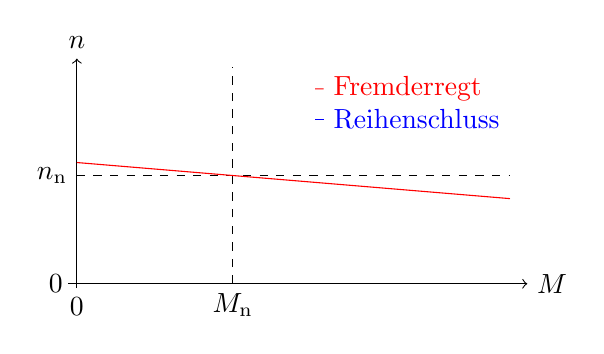
\begin{tikzpicture}[domain=0.9:10, samples=92, scale=0.55]
					\draw[->] (-0.2,0) -- (10.4,0) node[right] {$M$};
					\draw[->] (0,-0.1) -- (0,5.2) node[above] {$n$};	
					\draw (0,-0.1) node[below] {$0$};
					\draw (-0.1,0) node[left] {$0$};				
					\draw[blue, smooth] plot[id=Gleichstrommaschine1] function{ 1.5/ sqrt(0.1*x) };										
					\draw[dashed] (0,2.5) -- (10,2.5);											
					\draw[dashed] (3.6,0) -- (3.6,5);
					\draw (3.6,0) node[below] {$M_\mathrm{n}$};
					\draw (0,2.5) node[left] {$n_\mathrm{n}$};
					\draw[red] (0,2.8) -- (10,1.966666)  (5.5,4.5) -- (5.7,4.5) node[right]{Fremderregt};
					\draw[blue] (5.5,3.8) -- (5.7,3.8) node[right]{Reihenschluss};
					\end{tikzpicture}
				}{Kennlinien von Gleichstrommaschinen}
			}	
	\end{columns}
\end{frame}





